% Created by tikzDevice version 0.12.6 on 2026-02-22 21:43:39
% !TEX encoding = UTF-8 Unicode
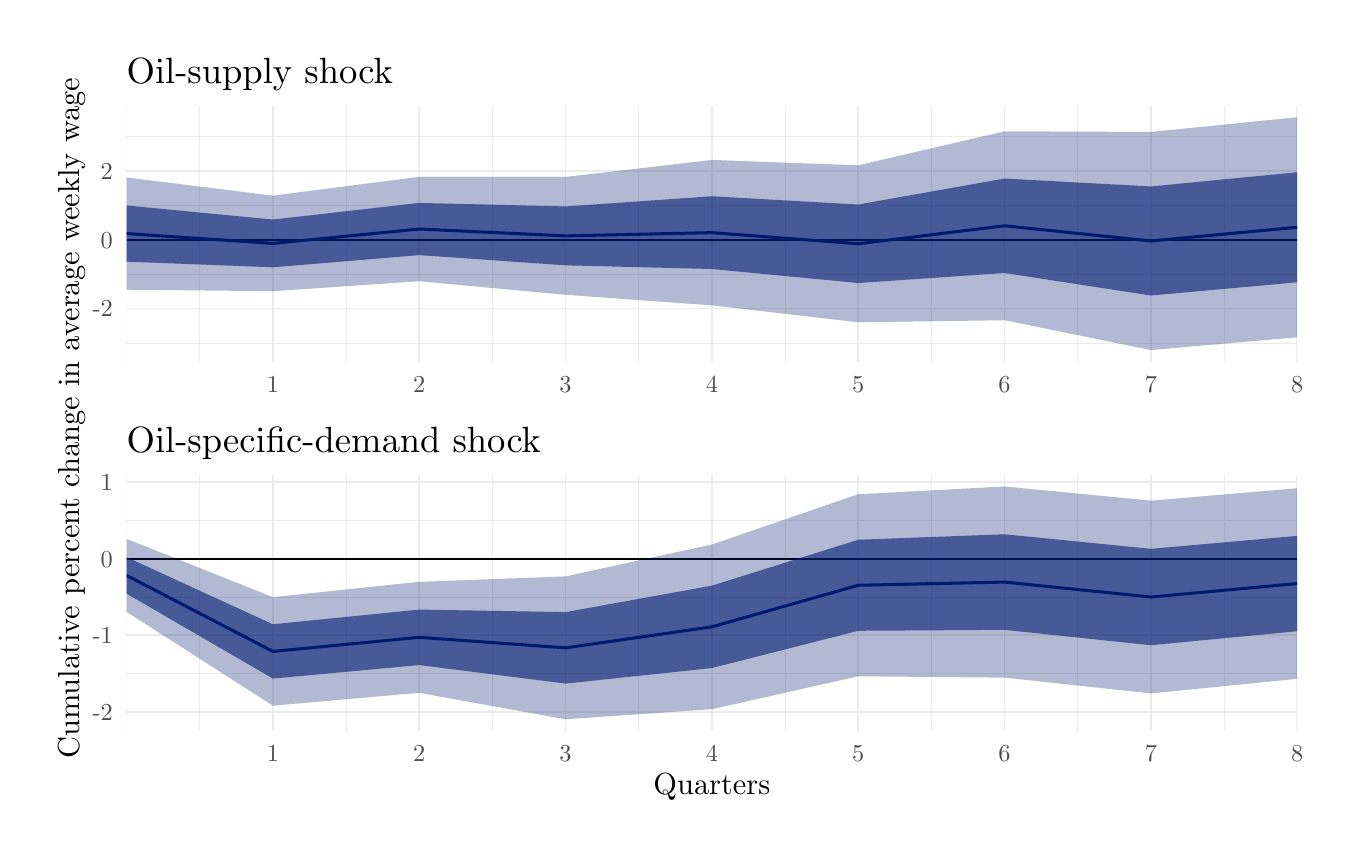
\begin{tikzpicture}[x=1pt,y=1pt]
\definecolor{fillColor}{RGB}{255,255,255}
\path[use as bounding box,fill=fillColor,fill opacity=0.00] (0,0) rectangle (469.75,290.32);
\begin{scope}
\path[clip] (  0.00,  0.00) rectangle (469.75,290.32);
\definecolor{drawColor}{RGB}{255,255,255}
\definecolor{fillColor}{RGB}{255,255,255}

\path[draw=drawColor,line width= 0.6pt,line join=round,line cap=round,fill=fillColor] (  0.00,  0.00) rectangle (469.76,290.32);
\end{scope}
\begin{scope}
\path[clip] ( 35.75,169.62) rectangle (458.75,262.17);
\definecolor{drawColor}{gray}{0.92}

\path[draw=drawColor,line width= 0.3pt,line join=round] ( 35.75,176.38) --
	(458.75,176.38);

\path[draw=drawColor,line width= 0.3pt,line join=round] ( 35.75,201.24) --
	(458.75,201.24);

\path[draw=drawColor,line width= 0.3pt,line join=round] ( 35.75,226.10) --
	(458.75,226.10);

\path[draw=drawColor,line width= 0.3pt,line join=round] ( 35.75,250.96) --
	(458.75,250.96);

\path[draw=drawColor,line width= 0.3pt,line join=round] ( 35.75,169.62) --
	( 35.75,262.17);

\path[draw=drawColor,line width= 0.3pt,line join=round] ( 62.18,169.62) --
	( 62.18,262.17);

\path[draw=drawColor,line width= 0.3pt,line join=round] (115.06,169.62) --
	(115.06,262.17);

\path[draw=drawColor,line width= 0.3pt,line join=round] (167.94,169.62) --
	(167.94,262.17);

\path[draw=drawColor,line width= 0.3pt,line join=round] (220.81,169.62) --
	(220.81,262.17);

\path[draw=drawColor,line width= 0.3pt,line join=round] (273.69,169.62) --
	(273.69,262.17);

\path[draw=drawColor,line width= 0.3pt,line join=round] (326.56,169.62) --
	(326.56,262.17);

\path[draw=drawColor,line width= 0.3pt,line join=round] (379.44,169.62) --
	(379.44,262.17);

\path[draw=drawColor,line width= 0.3pt,line join=round] (432.32,169.62) --
	(432.32,262.17);

\path[draw=drawColor,line width= 0.6pt,line join=round] ( 35.75,188.81) --
	(458.75,188.81);

\path[draw=drawColor,line width= 0.6pt,line join=round] ( 35.75,213.67) --
	(458.75,213.67);

\path[draw=drawColor,line width= 0.6pt,line join=round] ( 35.75,238.53) --
	(458.75,238.53);

\path[draw=drawColor,line width= 0.6pt,line join=round] ( 88.62,169.62) --
	( 88.62,262.17);

\path[draw=drawColor,line width= 0.6pt,line join=round] (141.50,169.62) --
	(141.50,262.17);

\path[draw=drawColor,line width= 0.6pt,line join=round] (194.37,169.62) --
	(194.37,262.17);

\path[draw=drawColor,line width= 0.6pt,line join=round] (247.25,169.62) --
	(247.25,262.17);

\path[draw=drawColor,line width= 0.6pt,line join=round] (300.13,169.62) --
	(300.13,262.17);

\path[draw=drawColor,line width= 0.6pt,line join=round] (353.00,169.62) --
	(353.00,262.17);

\path[draw=drawColor,line width= 0.6pt,line join=round] (405.88,169.62) --
	(405.88,262.17);

\path[draw=drawColor,line width= 0.6pt,line join=round] (458.75,169.62) --
	(458.75,262.17);
\definecolor{drawColor}{RGB}{0,0,0}

\path[draw=drawColor,line width= 0.6pt,line join=round] ( 35.75,213.67) -- (458.75,213.67);
\definecolor{drawColor}{RGB}{0,26,112}

\path[draw=drawColor,line width= 1.1pt,line join=round] ( 35.75,215.91) --
	( 88.62,212.36) --
	(141.50,217.56) --
	(194.37,215.08) --
	(247.25,216.25) --
	(300.13,212.23) --
	(353.00,218.73) --
	(405.88,213.23) --
	(458.75,218.20);
\definecolor{fillColor}{RGB}{0,26,112}

\path[fill=fillColor,fill opacity=0.60] ( 35.75,226.06) --
	( 88.62,220.99) --
	(141.50,226.99) --
	(194.37,225.72) --
	(247.25,229.39) --
	(300.13,226.41) --
	(353.00,235.80) --
	(405.88,232.94) --
	(458.75,238.08) --
	(458.75,198.32) --
	(405.88,193.53) --
	(353.00,201.67) --
	(300.13,198.05) --
	(247.25,203.11) --
	(194.37,204.44) --
	(141.50,208.13) --
	( 88.62,203.73) --
	( 35.75,205.77) --
	cycle;

\path[] ( 35.75,226.06) --
	( 88.62,220.99) --
	(141.50,226.99) --
	(194.37,225.72) --
	(247.25,229.39) --
	(300.13,226.41) --
	(353.00,235.80) --
	(405.88,232.94) --
	(458.75,238.08);

\path[] (458.75,198.32) --
	(405.88,193.53) --
	(353.00,201.67) --
	(300.13,198.05) --
	(247.25,203.11) --
	(194.37,204.44) --
	(141.50,208.13) --
	( 88.62,203.73) --
	( 35.75,205.77);
\definecolor{fillColor}{RGB}{0,26,112}

\path[fill=fillColor,fill opacity=0.30] ( 35.75,236.20) --
	( 88.62,229.62) --
	(141.50,236.42) --
	(194.37,236.37) --
	(247.25,242.53) --
	(300.13,240.58) --
	(353.00,252.87) --
	(405.88,252.64) --
	(458.75,257.96) --
	(458.75,178.44) --
	(405.88,173.82) --
	(353.00,184.60) --
	(300.13,183.87) --
	(247.25,189.97) --
	(194.37,193.79) --
	(141.50,198.69) --
	( 88.62,195.10) --
	( 35.75,195.63) --
	cycle;

\path[] ( 35.75,236.20) --
	( 88.62,229.62) --
	(141.50,236.42) --
	(194.37,236.37) --
	(247.25,242.53) --
	(300.13,240.58) --
	(353.00,252.87) --
	(405.88,252.64) --
	(458.75,257.96);

\path[] (458.75,178.44) --
	(405.88,173.82) --
	(353.00,184.60) --
	(300.13,183.87) --
	(247.25,189.97) --
	(194.37,193.79) --
	(141.50,198.69) --
	( 88.62,195.10) --
	( 35.75,195.63);
\end{scope}
\begin{scope}
\path[clip] (  0.00,  0.00) rectangle (469.75,290.32);
\definecolor{drawColor}{gray}{0.30}

\node[text=drawColor,anchor=base east,inner sep=0pt, outer sep=0pt, scale=  0.88] at ( 30.80,185.78) {-2};

\node[text=drawColor,anchor=base east,inner sep=0pt, outer sep=0pt, scale=  0.88] at ( 30.80,210.64) {0};

\node[text=drawColor,anchor=base east,inner sep=0pt, outer sep=0pt, scale=  0.88] at ( 30.80,235.50) {2};
\end{scope}
\begin{scope}
\path[clip] (  0.00,  0.00) rectangle (469.75,290.32);
\definecolor{drawColor}{gray}{0.30}

\node[text=drawColor,anchor=base,inner sep=0pt, outer sep=0pt, scale=  0.88] at ( 88.62,158.61) {1};

\node[text=drawColor,anchor=base,inner sep=0pt, outer sep=0pt, scale=  0.88] at (141.50,158.61) {2};

\node[text=drawColor,anchor=base,inner sep=0pt, outer sep=0pt, scale=  0.88] at (194.37,158.61) {3};

\node[text=drawColor,anchor=base,inner sep=0pt, outer sep=0pt, scale=  0.88] at (247.25,158.61) {4};

\node[text=drawColor,anchor=base,inner sep=0pt, outer sep=0pt, scale=  0.88] at (300.13,158.61) {5};

\node[text=drawColor,anchor=base,inner sep=0pt, outer sep=0pt, scale=  0.88] at (353.00,158.61) {6};

\node[text=drawColor,anchor=base,inner sep=0pt, outer sep=0pt, scale=  0.88] at (405.88,158.61) {7};

\node[text=drawColor,anchor=base,inner sep=0pt, outer sep=0pt, scale=  0.88] at (458.75,158.61) {8};
\end{scope}
\begin{scope}
\path[clip] (  0.00,  0.00) rectangle (469.75,290.32);
\definecolor{drawColor}{RGB}{0,0,0}

\node[text=drawColor,anchor=base west,inner sep=0pt, outer sep=0pt, scale=  1.32] at ( 35.75,270.23) {Oil-supply shock};
\end{scope}
\begin{scope}
\path[clip] ( 35.75, 36.19) rectangle (458.75,128.74);
\definecolor{drawColor}{gray}{0.92}

\path[draw=drawColor,line width= 0.3pt,line join=round] ( 35.75, 56.95) --
	(458.75, 56.95);

\path[draw=drawColor,line width= 0.3pt,line join=round] ( 35.75, 84.60) --
	(458.75, 84.60);

\path[draw=drawColor,line width= 0.3pt,line join=round] ( 35.75,112.25) --
	(458.75,112.25);

\path[draw=drawColor,line width= 0.3pt,line join=round] ( 35.75, 36.19) --
	( 35.75,128.74);

\path[draw=drawColor,line width= 0.3pt,line join=round] ( 62.18, 36.19) --
	( 62.18,128.74);

\path[draw=drawColor,line width= 0.3pt,line join=round] (115.06, 36.19) --
	(115.06,128.74);

\path[draw=drawColor,line width= 0.3pt,line join=round] (167.94, 36.19) --
	(167.94,128.74);

\path[draw=drawColor,line width= 0.3pt,line join=round] (220.81, 36.19) --
	(220.81,128.74);

\path[draw=drawColor,line width= 0.3pt,line join=round] (273.69, 36.19) --
	(273.69,128.74);

\path[draw=drawColor,line width= 0.3pt,line join=round] (326.56, 36.19) --
	(326.56,128.74);

\path[draw=drawColor,line width= 0.3pt,line join=round] (379.44, 36.19) --
	(379.44,128.74);

\path[draw=drawColor,line width= 0.3pt,line join=round] (432.32, 36.19) --
	(432.32,128.74);

\path[draw=drawColor,line width= 0.6pt,line join=round] ( 35.75, 43.13) --
	(458.75, 43.13);

\path[draw=drawColor,line width= 0.6pt,line join=round] ( 35.75, 70.78) --
	(458.75, 70.78);

\path[draw=drawColor,line width= 0.6pt,line join=round] ( 35.75, 98.43) --
	(458.75, 98.43);

\path[draw=drawColor,line width= 0.6pt,line join=round] ( 35.75,126.07) --
	(458.75,126.07);

\path[draw=drawColor,line width= 0.6pt,line join=round] ( 88.62, 36.19) --
	( 88.62,128.74);

\path[draw=drawColor,line width= 0.6pt,line join=round] (141.50, 36.19) --
	(141.50,128.74);

\path[draw=drawColor,line width= 0.6pt,line join=round] (194.37, 36.19) --
	(194.37,128.74);

\path[draw=drawColor,line width= 0.6pt,line join=round] (247.25, 36.19) --
	(247.25,128.74);

\path[draw=drawColor,line width= 0.6pt,line join=round] (300.13, 36.19) --
	(300.13,128.74);

\path[draw=drawColor,line width= 0.6pt,line join=round] (353.00, 36.19) --
	(353.00,128.74);

\path[draw=drawColor,line width= 0.6pt,line join=round] (405.88, 36.19) --
	(405.88,128.74);

\path[draw=drawColor,line width= 0.6pt,line join=round] (458.75, 36.19) --
	(458.75,128.74);
\definecolor{drawColor}{RGB}{0,0,0}

\path[draw=drawColor,line width= 0.6pt,line join=round] ( 35.75, 98.43) -- (458.75, 98.43);
\definecolor{drawColor}{RGB}{0,26,112}

\path[draw=drawColor,line width= 1.1pt,line join=round] ( 35.75, 92.39) --
	( 88.62, 64.93) --
	(141.50, 70.02) --
	(194.37, 66.22) --
	(247.25, 73.81) --
	(300.13, 88.83) --
	(353.00, 89.99) --
	(405.88, 84.59) --
	(458.75, 89.45);
\definecolor{fillColor}{RGB}{0,26,112}

\path[fill=fillColor,fill opacity=0.60] ( 35.75, 98.99) --
	( 88.62, 74.73) --
	(141.50, 80.05) --
	(194.37, 79.13) --
	(247.25, 88.69) --
	(300.13,105.28) --
	(353.00,107.26) --
	(405.88,102.00) --
	(458.75,106.67) --
	(458.75, 72.23) --
	(405.88, 67.17) --
	(353.00, 72.72) --
	(300.13, 72.38) --
	(247.25, 58.93) --
	(194.37, 53.31) --
	(141.50, 60.00) --
	( 88.62, 55.12) --
	( 35.75, 85.80) --
	cycle;

\path[] ( 35.75, 98.99) --
	( 88.62, 74.73) --
	(141.50, 80.05) --
	(194.37, 79.13) --
	(247.25, 88.69) --
	(300.13,105.28) --
	(353.00,107.26) --
	(405.88,102.00) --
	(458.75,106.67);

\path[] (458.75, 72.23) --
	(405.88, 67.17) --
	(353.00, 72.72) --
	(300.13, 72.38) --
	(247.25, 58.93) --
	(194.37, 53.31) --
	(141.50, 60.00) --
	( 88.62, 55.12) --
	( 35.75, 85.80);
\definecolor{fillColor}{RGB}{0,26,112}

\path[fill=fillColor,fill opacity=0.30] ( 35.75,105.58) --
	( 88.62, 84.54) --
	(141.50, 90.08) --
	(194.37, 92.04) --
	(247.25,103.56) --
	(300.13,121.73) --
	(353.00,124.53) --
	(405.88,119.41) --
	(458.75,123.89) --
	(458.75, 55.01) --
	(405.88, 49.76) --
	(353.00, 55.45) --
	(300.13, 55.94) --
	(247.25, 44.06) --
	(194.37, 40.39) --
	(141.50, 49.97) --
	( 88.62, 45.32) --
	( 35.75, 79.20) --
	cycle;

\path[] ( 35.75,105.58) --
	( 88.62, 84.54) --
	(141.50, 90.08) --
	(194.37, 92.04) --
	(247.25,103.56) --
	(300.13,121.73) --
	(353.00,124.53) --
	(405.88,119.41) --
	(458.75,123.89);

\path[] (458.75, 55.01) --
	(405.88, 49.76) --
	(353.00, 55.45) --
	(300.13, 55.94) --
	(247.25, 44.06) --
	(194.37, 40.39) --
	(141.50, 49.97) --
	( 88.62, 45.32) --
	( 35.75, 79.20);
\end{scope}
\begin{scope}
\path[clip] (  0.00,  0.00) rectangle (469.75,290.32);
\definecolor{drawColor}{gray}{0.30}

\node[text=drawColor,anchor=base east,inner sep=0pt, outer sep=0pt, scale=  0.88] at ( 30.80, 40.10) {-2};

\node[text=drawColor,anchor=base east,inner sep=0pt, outer sep=0pt, scale=  0.88] at ( 30.80, 67.75) {-1};

\node[text=drawColor,anchor=base east,inner sep=0pt, outer sep=0pt, scale=  0.88] at ( 30.80, 95.40) {0};

\node[text=drawColor,anchor=base east,inner sep=0pt, outer sep=0pt, scale=  0.88] at ( 30.80,123.04) {1};
\end{scope}
\begin{scope}
\path[clip] (  0.00,  0.00) rectangle (469.75,290.32);
\definecolor{drawColor}{gray}{0.30}

\node[text=drawColor,anchor=base,inner sep=0pt, outer sep=0pt, scale=  0.88] at ( 88.62, 25.18) {1};

\node[text=drawColor,anchor=base,inner sep=0pt, outer sep=0pt, scale=  0.88] at (141.50, 25.18) {2};

\node[text=drawColor,anchor=base,inner sep=0pt, outer sep=0pt, scale=  0.88] at (194.37, 25.18) {3};

\node[text=drawColor,anchor=base,inner sep=0pt, outer sep=0pt, scale=  0.88] at (247.25, 25.18) {4};

\node[text=drawColor,anchor=base,inner sep=0pt, outer sep=0pt, scale=  0.88] at (300.13, 25.18) {5};

\node[text=drawColor,anchor=base,inner sep=0pt, outer sep=0pt, scale=  0.88] at (353.00, 25.18) {6};

\node[text=drawColor,anchor=base,inner sep=0pt, outer sep=0pt, scale=  0.88] at (405.88, 25.18) {7};

\node[text=drawColor,anchor=base,inner sep=0pt, outer sep=0pt, scale=  0.88] at (458.75, 25.18) {8};
\end{scope}
\begin{scope}
\path[clip] (  0.00,  0.00) rectangle (469.75,290.32);
\definecolor{drawColor}{RGB}{0,0,0}

\node[text=drawColor,anchor=base,inner sep=0pt, outer sep=0pt, scale=  1.10] at (247.25, 13.14) {Quarters};
\end{scope}
\begin{scope}
\path[clip] (  0.00,  0.00) rectangle (469.75,290.32);
\definecolor{drawColor}{RGB}{0,0,0}

\node[text=drawColor,rotate= 90.00,anchor=base,inner sep=0pt, outer sep=0pt, scale=  1.10] at ( 18.58,149.18) {Cumulative percent change in average weekly wage};
\end{scope}
\begin{scope}
\path[clip] (  0.00,  0.00) rectangle (469.75,290.32);
\definecolor{drawColor}{RGB}{0,0,0}

\node[text=drawColor,anchor=base west,inner sep=0pt, outer sep=0pt, scale=  1.32] at ( 35.75,136.80) {Oil-specific-demand shock};
\end{scope}
\end{tikzpicture}
